% Created 2020-07-03 Fri 17:25
% Intended LaTeX compiler: pdflatex
\documentclass[a4paper]{apa6}
\usepackage[utf8]{inputenc}
\usepackage[T1]{fontenc}
\usepackage{graphicx}
\usepackage{grffile}
\usepackage{longtable}
\usepackage{wrapfig}
\usepackage{rotating}
\usepackage[normalem]{ulem}
\usepackage{amsmath}
\usepackage{textcomp}
\usepackage{amssymb}
\usepackage{capt-of}
\usepackage{hyperref}
\affiliation{King's College London}
\shorttitle{Multi-scale modelling of carbon migration in iron}
\usepackage{breakcites}
\usepackage{apacite}
\usepackage{paralist}
\let\itemize\compactitem
\let\description\compactdesc
\let\enumerate\compactenum
\author{Tigany Zarrouk}
\date{\today}
\title{Multi-scale investigation of dislocation mediated carbon migration in iron}
\hypersetup{
 pdfauthor={Tigany Zarrouk},
 pdftitle={Multi-scale investigation of dislocation mediated carbon migration in iron},
 pdfkeywords={},
 pdfsubject={},
 pdfcreator={Emacs 26.3 (Org mode 9.1.9)}, 
 pdflang={English}}
\begin{document}

\maketitle
\tableofcontents

\begin{abstract}

*Abstract*

We investigate the validity of a dislocation-assisted carbon migration
mechanism underpinning the formation of dark etching regions in
bearing steels undergoing high-cycle fatigue through use of a
multi-scale approach: from quantum mechanics,
to stochastic simulations. We start from tight binding simulations of
$1/3\langle 111 \rangle$ screw dislocations to obtain the 2-d Peierls
potential and Fe-C binding energies. These become ingredients for a line-tension
model of the $1/3\langle 111 \rangle$ screw dislocation to obtain the kink-pair formation
energy as a function of stress and carbon concentration. Finally,
3-d kinetic Monte-Carlo simulations of dislocations in an environment
of carbon are used to ascertain which temperature and stress regimes
dislocation-assisted carbon migration is a valid mechanism. 

\end{abstract}


\section{Introduction}
\label{sec:org9bf46eb}

\section{Computational Method}
\label{sec:org4605623}

\begin{itemize}
\item Use tight-binding model of Paxton and Elsaetter \cite{Paxton2013}.
\item Generate dislocations using anisotropic elasticity theory.
\item Create clusters of dislocations in both easy and hard core
configurations.
\item Place carbon in octahedral sites around the core
\item Calculate corrections (ZPE etc)
\end{itemize}


\section{Results}
\label{sec:orgb186146}

\subsection{Hard and easy core relaxations}
\label{sec:org266eb33}

Plot of dislocation energy as function of cluster size. 
\begin{center}
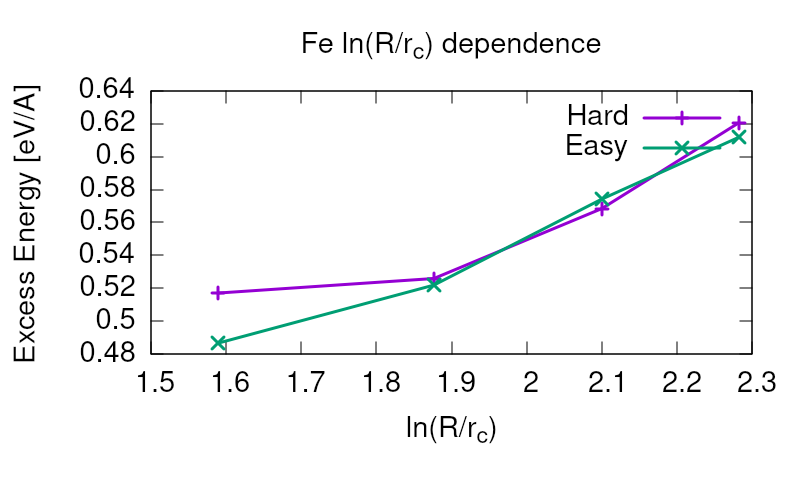
\includegraphics[width=.9\linewidth]{/home/tigany/Documents/docs/Management/Images/img_fe_size_dependence_on_log_of_core_radius.png}
\end{center}



     \begin{table}	
    \begin{tabular}{cc}
        \small  Initial  & Final \\ 
	     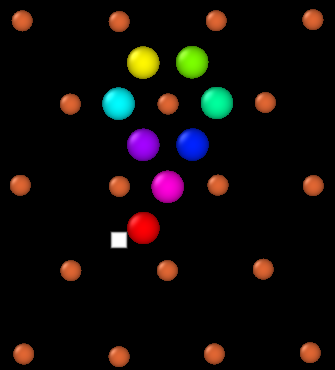
\includegraphics[width=0.24\textwidth]{../Images/easy_core_initial_all_fe_octahedral_sites_with_core.png} &
	           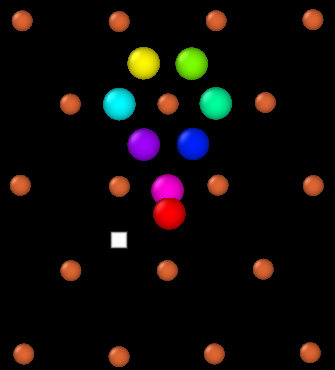
\includegraphics[width=0.24\textwidth]{../Images/easy_core_final_all_fe_octahedral_sites_with_core.png}  \\
	     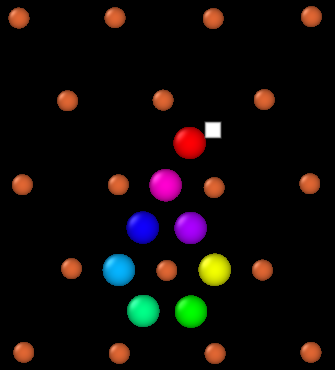
\includegraphics[width=0.24\textwidth]{../Images/hard_core_initial_all_fe_octahedral_sites_with_core.png} &
	           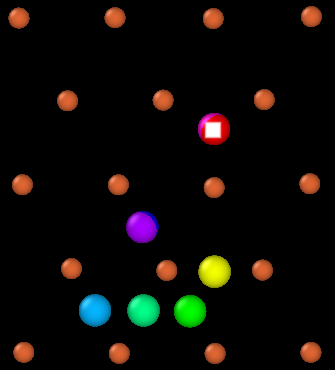
\includegraphics[width=0.24\textwidth]{../Images/hard_core_final_all_fe_octahedral_sites_with_core.png}  \\
		   
    	      \end{tabular}		
\caption{ Initial and final octahedral sites for the easy core (first row) and the hard core (second row). As shown by Ventelon cite:Ventelon2015, the first and second closest octahedral sites to the hard core have their minimum energy inside the hard core, but we do not find that the easy core reconstructs into a hard core, with these same sites. }
    \end{table}


Following the paper by Itakura
\cite{itakura13_effec_hydrog_atoms_screw_disloc} we calculated the
binding energy of carbon each of the screw dislocation cores. 

The solution energy is given by 
\[ E_s = E_{\text{d + C}} - E_{\text{d}} - E_{\text{C oct.}}, \]
where \(E_{\text{d + C}}\) is the total energy of a relaxed cluster with a
carbon interstitial and a dislocation, \(E_{\text{d}}\) is the total
energy of a relaxed cluster with a dislocation and \(E_{\text{C
    oct.}}\) is the total energy of relaxed a cluster with a single carbon in
an octahedral site.

The zero-point energy is calculated as in Itakura. A 3x3 Hessian
matrix is constructed by taking the numerical derivative of the
forces observed on the carbon atom after displacement by \(\pm 0.015 \AA\) in each of the \(X\), \(Y\) and \(Z\)
directions. The zero-point energy is given by

\[ E_z = \frac{1}{2} \sum_{i=1}^3 \frac{h}{2\pi} \sqrt{ k_i /
    m_{\text{C}} },  \]
where \(k_i\) are the eigenvalues of the Hessian and \(m_\text{C}\) is
the mass of carbon. 

The ZPE corrected solution energy is given by 
\[ E^{\text{Z}}_{s} = E_s + E_z - E_{z\text{C oct.}},  \]

where \(E_{z\text{C oct.}} = 202.5 meV\) is the zero-point energy of carbon
situated in an octahedral site in a perfect cluster of the same size. 

Table of relaxed energies.  

\begin{center}
\begin{tabular}{lrrrrr}
Site Type & \(E_{\text{d + C}} - E_{\text{d}}\)) & \(E_s\) & \(E_z - E_{z\text{ C oct.}}\) \(meV\) & \(E^b_z\) \(meV\) & distance from core\\
\hline
E1 & -0.89299636 & -0.05828365 & -17.8194 & -775.17 & 1.413699\\
E2 & -0.89300553 & -0.05829282 & -0.529601 & -792.585 & 1.732527\\
E3 & -0.84476459 & -0.01005188 & 2.47361 & -139.236 & 2.458179\\
E4 & -0.85151735 & -0.01680464 & 5.36252 & -234.001 & 3.001665\\
E5 & -0.89232261 & -0.0576099 & 7.63124 & -791.454 & 3.369997\\
E6 & -0.87856485 & -0.04385214 & 6.60286 & -603.242 & 4.129084\\
E7 & -0.86299687 & -0.02828416 & 3.21964 & -388.045 & 4.703422\\
E8 & -0.84773572 & -0.01302301 & 0.35220 & -177.539 & 4.409563\\
H1/H2 & -0.93009177 & -0.09537906 & -6.39993 & -1291.3 & 0.006472\\
H3/H4 & -0.88549598 & -0.05078327 & 7.3888 & -698.331 & 2.960187\\
H5 & -0.86857644 & -0.03386373 & 6.5459 & -467.286 & 5.287079\\
H6 & -0.85757695 & -0.02286424 & 4.6842 & -315.768 & 4.746490\\
H7 & -0.8643446 & -0.02963189 & 6.1659 & -409.328 & 4.483550\\
H8 & -0.82596378 & 8.74893\,(-3) & 4.7335 & 114.302 & 3.480325\\
\end{tabular}
\end{center}



Distance dependence of binding energies. 




\section{Bibliography}
\label{sec:org0595511}
\label{org172d722}

\bibliographystyle{apacite}
\bibliography{../bibliography/org-refs}
\end{document}